\section{Zero knowledge}
Špeciálnym prípadom interaktívnych dokazovacích systémov sú takzvané
bezznalostné dôkazy. Základná myšlienka sa dá ilustrovať na príklade 
"Alibaba a jaskyňa tajomstiev".

Alibaba na svojich potulkách narazil (alebo skôr naďabil) na jaskyňu,
ktorá má čarovnú stenu. Táto stena sa na vyslovenie čarovnej formuly
otvorí a prepustí človeka na druhú stranu. Po dlhšom skúmaní
prišiel na to, že jaskyňa vyzerá ako na obr. \ref{fig:alibaba}. Pretože v
jaskyni neboli žiadne poklady (alebo boli, ale niekto ich stihol
vybrať skorej), Alibaba sa rozhodol zbohatnúť na TV show.
Bude ukazovať, že vie tajnú formulku a nafilmujú ho pritom. Nechce ale
prezradiť tajomstvo zvyšku sveta.

\begin{figure}[htp]
    \centering
    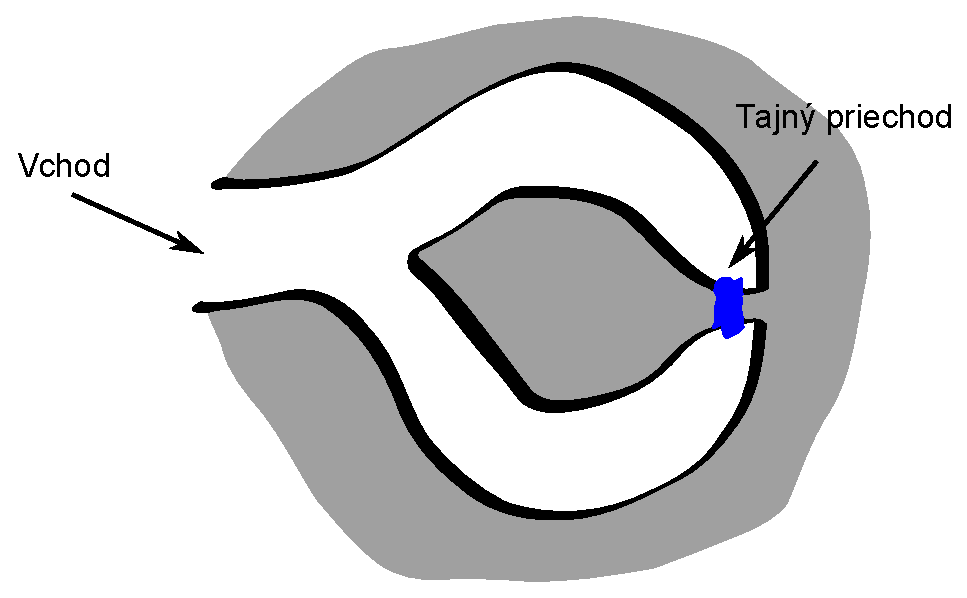
\includegraphics[scale=0.4]{img/x/alibaba}
    
    \label{fig:alibaba}
    \caption{Alibabova jaskyňa}
\end{figure}

Preto sa s filmármi dohodol na nasledujúcom postupe - vôjde do jaskyne
sám. Následne dnu vojde aj filmový štáb a ten zakričí Aladinovi, z
ktorej strany má dôjsť. Ten na demonštráciu znalosti prechádzania cez
steny vyjde zo správnej strany.

Poučenie z príbehu: Môžeme si všimnúť, že Aladin nikomu neprezradí
svoje tajomstvo. Zároveň ale presvedčí štáb o tom, že cez tie steny
chodí, pretože inak by si musel vedieť niekoľkokrát po sebe správne
tipnúť, čo sa mu rozhodnú zakričať, keď dôjdu na rázcestie.
Dôkaz má ale aj ďalšiu vlastnosť - Aladin síce presvedčil štáb, ale
môže presvedčiť aj divákov? Nie. Čo ak bolo napríklad video
"nastrihané" iba na dobré pokusy? Takémuto ``strihanie'' bude
vo formálnej definícii zodpovedať simulátor -- mohli by sme povedať,
že bude zastupovať šikovného strihača filmu, ktorý nepodarené pokusy
vystrihne.

Bezznalostné dokazovacie systémy sú preto také systémy, pri ktorých
dokazovateľ presvedčí overovateľa o svojej pravde bez toho aby mu
prezradil čokoľvek iné. Taktiež, ľubovoľný externý pozorovateľ
komunikácie nemá byť schopný odlíšiť reálny dôkaz od akéhosi
vykonštruovaného. 

\begin{definicia}[Zero knowledge]

Označme:
\begin{itemize}
\itemsep -1.2mm
    \item $V^*$ -- overovateľ (nečestný)
    \item $S^*$ -- simulátor, pravdepodobnostný stroj pracujúci
        v polynomiálnom čase
    \item $T(V^*, x)$ -- množina komunikácií na vstupe $x$
    \item $F(V^*, x)$ -- množina simulovaných komunikácií na vstupe $x$
    \item $p_t(x,y)$ -- pravdepodobnosť, že komunikácia na vstupe $x$
            bude $y$
    \item $p_f(x,y)$ -- pravdepodobnosť, že simulátor vygeneruje na
            vstupe $x$ komunikáciu $y$
\end{itemize}

Potom interaktívny dokazovací systém pre jazyk L je perfektné bezznalostný,
ak 
\begin{equation*}
    \forall V^*\ \exists S^*\ \forall x \in L \mbox{ platí }
        T(V^*, x) = F(V^*, x) \mbox{ a tiež } 
        \forall t \in T(V^*,x) \colon p_t(x,t) = p_f(x,t)
\end{equation*}

Teda ak simulátor vie generovať takú komunikáciu, ktorá má presne rovnaké rozloženie
pravdepodobnosti ako reálna komunikácia.
\end{definicia}

\begin{poznamka}
Pokiaľ sú distribúcie v množinách $T$ a $F$ nerozlíšiteľné
v polynomiálnom čase hovoríme, že systém je výpočtovo bezznalostný.
\end{poznamka}


\todo{zvysok, blackbox simulator}
\todo{ZK pre izomorfizmus}

\begin{poznamka}
    Na tomto mieste by sme upozornili čitateľa na fakt, že nami
    prezentovaný algoritmus v predchádzajúcej sekcii na neizomorfizmus grafov
    nie je bezznalostný.
    
    Prečo? Uvažujme falošného verifikátora $V'$,
    ktorý má graf $G$ a vie, že je izomorfný buď s $G_0$ alebo s
    $G_1$. V tomto prípade môže využiť provera $P$ ako orákulum na
    problém izomorfizmu grafov -- jednoducho mu pošle $G$, čo je
    validná správa a vráti sa mu index.

    No dobre. A ako súvisí to, že $V'$ vie niečo zistiť s definíciou
    bezznalosti, t.j. s existenciou simulátora? Jednoducho tak, že
    každý polynomiálny simulátor by musel vedieť simulovať komunikáciu
    $P$ s $V'$. Toto ale nemôže vedieť, pretože by sme vedeli v
    polynomiálnom čase riešiť izomorfizmus grafov, čo za predpokladu
    $P\neq NP$ nevieme. Preto dôkaz nie je bezznalostný z definície.
    Záverom teda môžeme usudzovať, že existencia polynomiálneho
    simulátora je naozaj ekvivalentná našej intuícii, čo to znamená
    "bezznalostný".

    Pre záujemcov o bezznalostný algoritmus pre neizomorfizmus grafov
    odporúčame prečítať \cite{nig}, kde je uvedené rozšírenie našeho
    postupu tak, aby $P$ nič neprezradil.
\end{poznamka}
